


This chapter contains routines for geometric optics solutions of reflection and refraction of rays at dielectric interfaces. All of these solutions are fundamentally based on Snell's law. Specifically, these routines will compute the reflection or reflection point on an interface given the positions of a source and observer as inputs. These algorithms are especially useful for radar scattering and subsurface imaging problems. Many of these solutions are well known. In general, very fast, and much better, codes for geometric optics can be found in the computer graphics literature.

This chapter contains: 1) routines for computing the reflection point on a plane and sphere, 2) derivations and two routines for solving for the refraction point through the plane: one is analytical, one is iterative, 3) an analytical solution for the refraction point on a circular interface given a pair of interior and exterior source and observation points, 4) a vectorized iterative solution for refraction through a circular interface, and 5) a simple coordinate transform for the solution for the refraction point on a sphere.



\section{Snell's Law}

Snell's law of refraction at a flat dielectric half-space is given by 
\eq{ \dfrac{\sin\theta_1}{\sin\theta_2} =  \dfrac{n_2}{n_1} }

\noindent where $\theta_1$ is the angle measured from normal in medium 1 with index of refraction, $n_1$, and $\theta_2$ is the angle measured from normal in medium 2 with index of refraction, $n_2$. Recall $n = \sqrt{\epsilon_r}$, where $\epsilon_r$ is the relative permittivity.


%
%\noindent This has the alternate form
%
%\[1 + \cot^2(\theta_t) = (1 + \cot^2(\theta_i)) \epsilon_r  \]



\section{Reflection Point - Flat Interface}

Here we find the ray-solution for the specular point for two arbitrary points above a flat surface. One point could be a source, the other a receiver. This can be solved a number of ways, including the image method or by enforcing equal incident and reflected angles relative to the normal of the specular point.

Let two points $\bb{r}_1$ and $\bb{r}_2$ be above a flat surface that is parallel to the XY plane at level $z = z_o$. Each half space has a different index of refraction. Define the following quantities 
\ea{h_1 &=&z_1-z_o \\
h_2 &=& z_2-z_o \\
L &=& \sqrt{(x_2-x_1)^2 + (y_2-y_1)^2} \\
\hat{u} &=& \dfrac{(x_2-x_1)  \hat{x} + (y_2-y_1)\hat{y}}{L} }

\noindent where $\hat{u}$ is the transverse unit vector from $\bb{r}_1$ and $\bb{r}_2$. Define the transverse distance from $\bb{r}_1$ to the reflection point as $u_1$ and from $\bb{r}_2$ to the reflection point as $u_2$.  Then for equal incident and reflected angles relative to normal
\ea{ \tan\theta &=& \dfrac{u_1}{h_1} \\
\tan\theta &=& \dfrac{u_2}{h_2} }

\begin{figure}[h] 
   \centering
   \includegraphics[width=3in]{ReflectionRefraction/Figures/reflectionPlane} 
   \caption{Geometry for the solution of the planar reflection point, $\bb{r}$, which is unknown.}
\end{figure}

Equating the sines, using the fact that $L = u_1 +u_2$, and solving for $u_1$, we get
\eq{u_1 = \dfrac{h_1 L}{(h_2 + h_1)} }

From which the reflection point $\bb{r}$ is found by reprojecting
\eq{\bb{r} = x_1 \hat{x} + y_1 \hat{y} + u_1 \hat{u} + z_o \hat{z_o}}

The routine \texttt{reflectionPlane} takes as input the two points, $\bb{r}_1$, $\bb{r}_2$, and the level of the plane, $z_o$, and returns the reflection point, $\bb{r}$, as well as $\theta$ and the lengths of the vectors $l_1$ and $l_2$.  This routine is vectorized for any number of pairs of source and receiver points.  


\begin{figure}[H] 
   \centering
   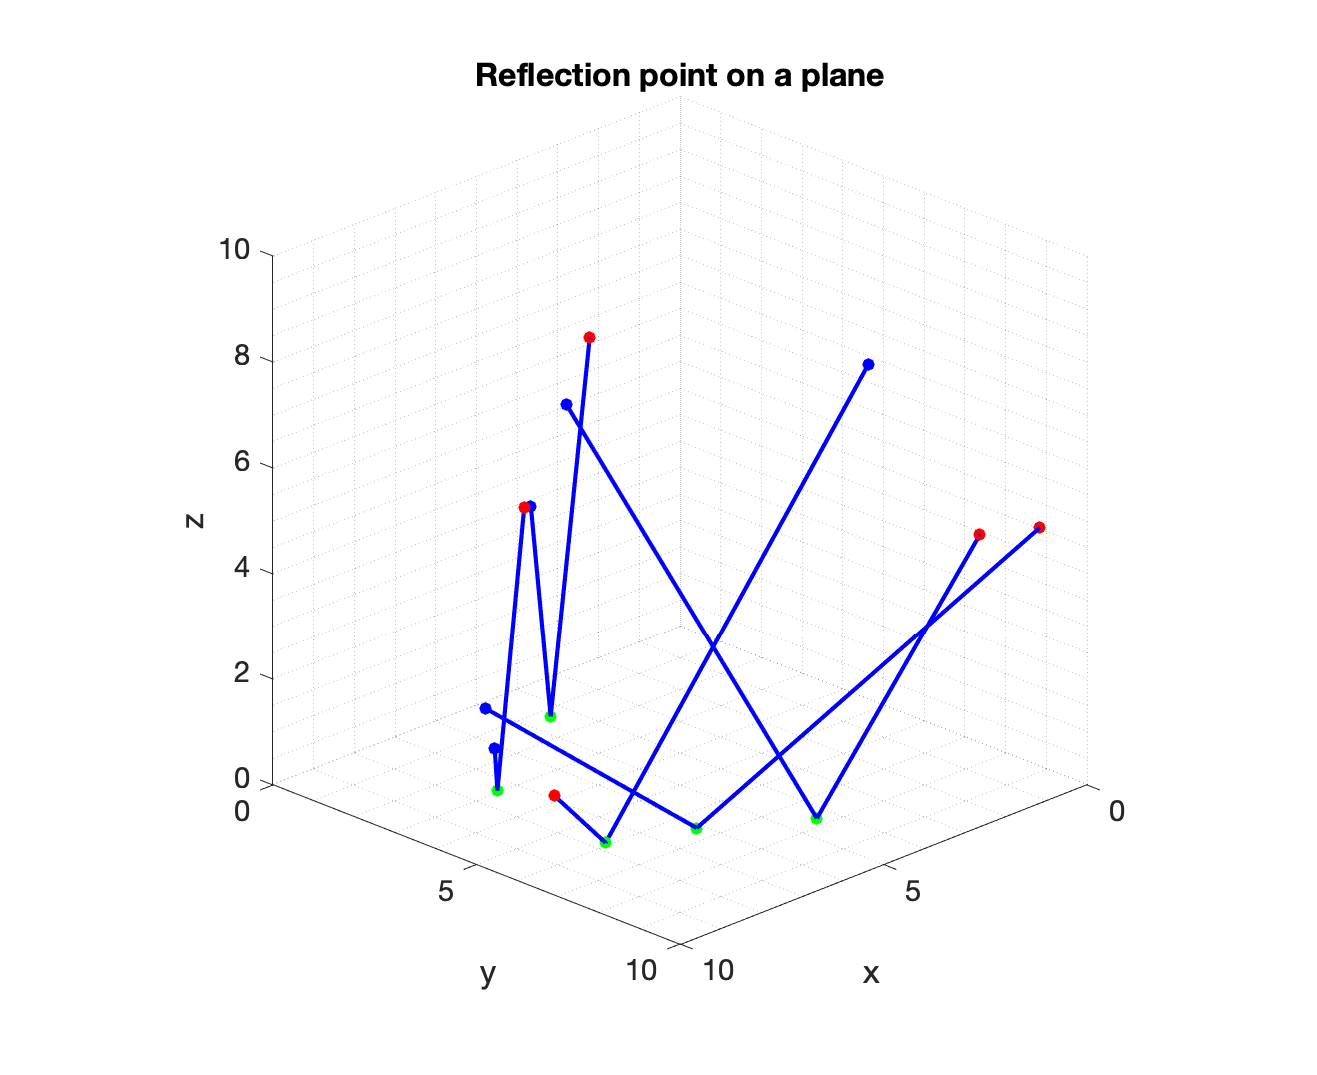
\includegraphics[width=4in]{ReflectionRefraction/Figures/reflectionraysplane} 
   \caption{Geometry for the solution of the planar reflection point, $\bb{r}$, which is unknown off a plane at level $z_o = 0$.}
\end{figure}


{\footnotesize
\VerbatimInput{\code/ReflectionRefraction/reflectionPlane.m}
}


\section{Reflection Point - Sphere}

Computing the reflection point on a sphere is often needed in Earth and planetary remote sensing, for example, when determining the specular point on a body between a source and receiver. The solution here is the one derived in \cite{reflection_sphere}, and summarized next. The reflection point on a circle can be found with this method by restricting the source and receiver points to a plane.

Let a sphere with radius $r$ be centered at the origin. $\bb{r}_1$ and $\bb{r}_2$ are radius-normalized vectors to exterior points 1 and 2, respectively, which can be a source and receiver.  Next, define the following coefficients 
\ea{a &=& \bb{r}_1\cdot\bb{r}_1 \\
b &=& \bb{r}_1\cdot\bb{r}_2 \\
c &=& \bb{r}_2\cdot\bb{r}_2}

After enforcing the reflection condition on the sphere, the solution comes from finding the roots of the following quartic polynomial
\eq{\sum_{n=0}^{4} a_n y^n = 0}
\ea{a_4 &=& 4c(ac-b^2) \\
a_3 &=& -4(ac-b^2) \\
a_2 &=& a+2b+c-4ac \\
a_1 &=& 2(a-b) \\
a_0 &=& a-1}

Once the roots are known, the positive roots with zero imaginary part are kept, call these $\bar{y}$. This is used to compute a second quantity
\eq{\bar{x} = \dfrac{-2 c \bar{y}^2 + \bar{y} + 1}{2 b \bar{y} + 1}}

The solution is the pair $(\bar{x},\bar{y})$ for which both are positive. Then the reflection point on the sphere is 
\eq{\bb{r} = r (\bar{x} \bb{r}_1 + \bar{y} \bb{r}_2 )}

\begin{figure}[h] 
   \centering
   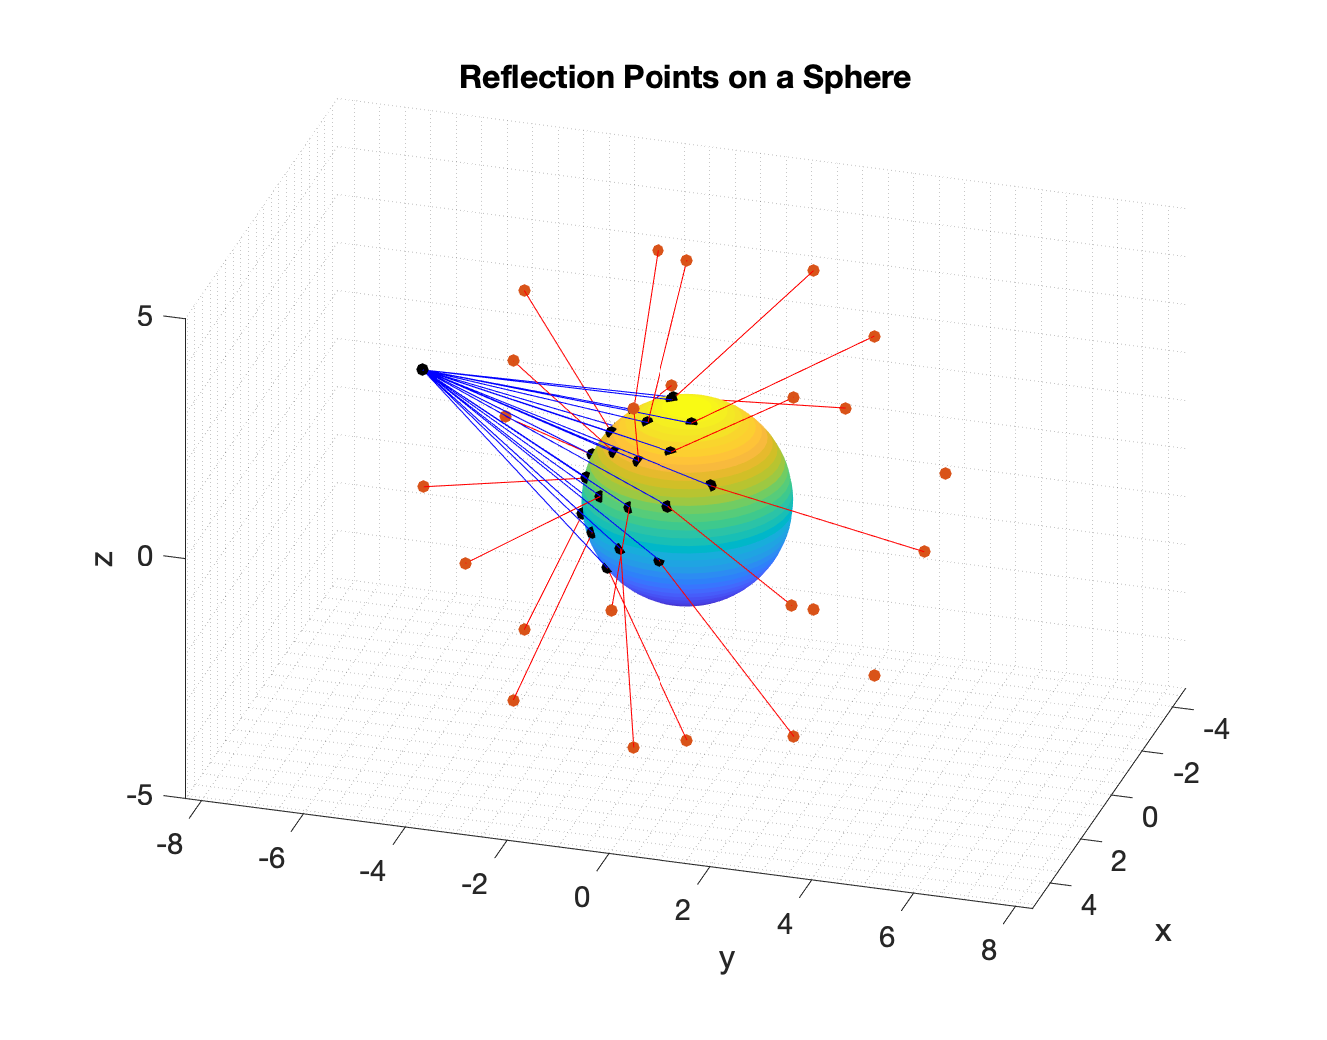
\includegraphics[width=4.5in]{ReflectionRefraction/Figures/reflectonraysphere} 
   \caption{Geometry for the reflection point on a sphere.}
\end{figure}

\paragraph{Line-Sphere Intersection} 

We exclude shadowed points by using the line-sphere intersection solution, \cite{linesphereintersect}. The equation for a line that originates at $\bb{r}_1$ and passes through $\bb{r}_2$ is
\eq{\bb{u}(l)  = \bb{r}_1 + l \hat{u} }

\noindent where $l$ is the distance along the line and $\hat{u}$ is
\eq{\hat{u} = \dfrac{\bb{r}_2 - \bb{r}_1}{\vert \bb{r}_2 - \bb{r}_1\vert}}

For a sphere with center, $\bb{c}$, and radius, $r$, the solutions for $l$ are
\ea{l &=& -\hat{u} \cdot(\bb{r}_1-\bb{c}) \pm \sqrt{\Delta} \\
\Delta &=& \left(\hat{u} \cdot(\bb{r}_1-\bb{c})\right)^2 - \left(\Vert \bb{r}_1 - \bb{c} \Vert^2 - r^2\right)}

If $\Delta < 0$ then there are no intersections. If $\Delta = 0$ then the line is tangent to the sphere. If $\Delta > 0$ then the line intersects the sphere at two places. In the last case, the reflection point is determined by checking which of the two intersection points is closer to the source.

\paragraph{Routine}
The routine \texttt{reflectionSphere} solves for the reflection point on a sphere that is centered at the origin. It takes as input the Cartesian points $\bb{r}_1$, $\bb{r}_2$, and the sphere radius, $r$, and returns the reflection point, $\bb{r}$, which lies on the surface of the sphere. The routine is vectorized to take multiple pairs of points at once, and returns \texttt{nan} if the points are shadowed or interior to the sphere. Shadowing is determined by the routine \texttt{lineIntersectSphere}, not copied here, that implements the line-sphere intersection solution above. 

{\footnotesize
\VerbatimInput{\code/ReflectionRefraction/reflectionSphere.m}
}


\section{Refraction Point - Flat Interface}

We derive two solutions for the refraction point through a flat dielectric interface given two arbitrary points on either side of the interface. The first solution is in terms of the roots of a quartic polynomial, \cite{heliere2007radio}. The second is an iterative algorithm, \cite{lei20202}. Practical applications of this are subsurface SAR processing, e.g. radar sounding through ice, ground penetrating radar, or through-wall imaging, where the propagation phase between two points across a dielectric interface needs to be computed for focusing. In these cases, the refraction point is really an intermediate result in order to obtain the incidence and transmission angles and propagation distances along the bent-ray path.  

The geometry is shown in Figure \ref{fig9a}. The dielectric interface is parallel to the $XY$ plane at level $z = z_o$. Let two points $\bb{r}_1$ and $\bb{r}_2$ be above and below the interface in mediums 1 and 2 each having an index of refraction, $n_1$ and $n_2$, respectively. Next define the following quantities, 
\ea{h &=& z_1 - z_o \\
d &=& z_2 - z_o \\
L &=& \sqrt{(x_2-x_1)^2 + (y_2-y_1)^2} \\
\hat{u} &=& \dfrac{(x_2-x_1)  \hat{x} + (y_2-y_1)\hat{y} }{L}}
 
\noindent \noindent where $h$ is the height of $\bb{r}_1$ above the interface, $d$ is the depth of $\bb{r}_2$ below the interface, $\hat{u}$ is the transverse unit vector and $L$ is the transverse distance from point 1 to point 2. Finally, $u$ is the transverse distance along $\hat{u}$ between the projection of $\br_1$ on the interface and the refraction point.
 
\begin{figure}[h] 
   \centering
   \includegraphics[width=3in]{ReflectionRefraction/Figures/refractionPlane} 
   \caption{Geometry for the solution of the planar refraction point, $\bb{r}$, which is unknown.}
   \label{fig9a}
\end{figure}

\subsubsection{Quartic Solution}
 
Start with the observations that 
\begin{eqnarray} 
\sin\theta_1 &=& \dfrac{u}{\sqrt{h^2 + u^2}} \nonumber \\
\sin\theta_2 &=& \dfrac{L-u}{\sqrt{d^2 + (L-u)^2}} \nonumber
\end{eqnarray}

These are equated though Snell's law
\eq{\dfrac{u}{\sqrt{h^2 + u^2}}   = \dfrac{n_2}{n_1}\dfrac{L-u}{\sqrt{d^2 + (L-u)^2}} } 

After squaring both sides, this can be rearranged as a fourth order polynomial in $u$:

\eq{ a u^4 + b u^3 + c u^2 + d u + e = 0}
\begin{eqnarray} 
a &=& n_1^2 - n_2^2 \nonumber \\
b &=& -2 L (n_1^2 - n_2^2) \nonumber \\
c &=& n_1^2(L^2  + d^2) - n_2^2( L^2 + h^2) \nonumber \\
d &=& 2 n_2^2 L h^2 \nonumber \\
e &=& -n_2^2 L^2 h^2  \nonumber
\end{eqnarray}

The roots can be found with a root finding algorithm or analytically. The solution is the positive real root for which $u < L$.  This solution is good for either $n_1 > n_2$ or $n_1 < n_2$. Once found, $u$ is reprojected to give the refraction point: 
\eq{\bb{r} = x_1 \hat{x} + y_1 \hat{y} + u \hat{u} + z_o \hat{z}}

\subsubsection{Iterative Solution}
For the iterative solution, we use the facts that  
\begin{eqnarray} 
u &=& h \tan \theta_1 \\
u &=& L - d \tan \theta_2 
\end{eqnarray}

Start with the straight-ray approximation for $\theta_1$, then with the addition of Snell's law, we can build the following iteration
\begin{eqnarray}
\textrm{Initialize:} \quad \quad \theta_1 &\leftarrow &\arctan\left( \dfrac{L}{h + d}\right) \ \nonumber \\
\textrm{Iterate:} \quad \quad\theta_2 &\leftarrow &\arcsin\left(\dfrac{n_1}{n_2} \sin\theta_1\right) \nonumber  \\
u & \leftarrow &L - d \tan\theta_2 \nonumber  \\
\theta_1 &\leftarrow&  \arctan\left( \dfrac{u}{h}\right) \nonumber
\end{eqnarray}

This is an alternating sequence for $u$ (and $\theta_1$, $\theta_2$). The physical interpretation is that the value of $u$ bounces closer to the true solution at every iteration. This is effectively a Newton iteration of the transcendental equation for $\theta_1$ without a nonlinear optimization algorithm. The solution is lightning fast (requiring maybe 10 iterations), when it works. The solution does not always converge, which happens when $h$ is too close to the interface relative to values of $d$ and $L$. In other words, this solution is valid when $d,L \le h$. Also, as written, this should only be used when $n_1 < n_2$.  

\begin{figure}[h] 
   \centering
   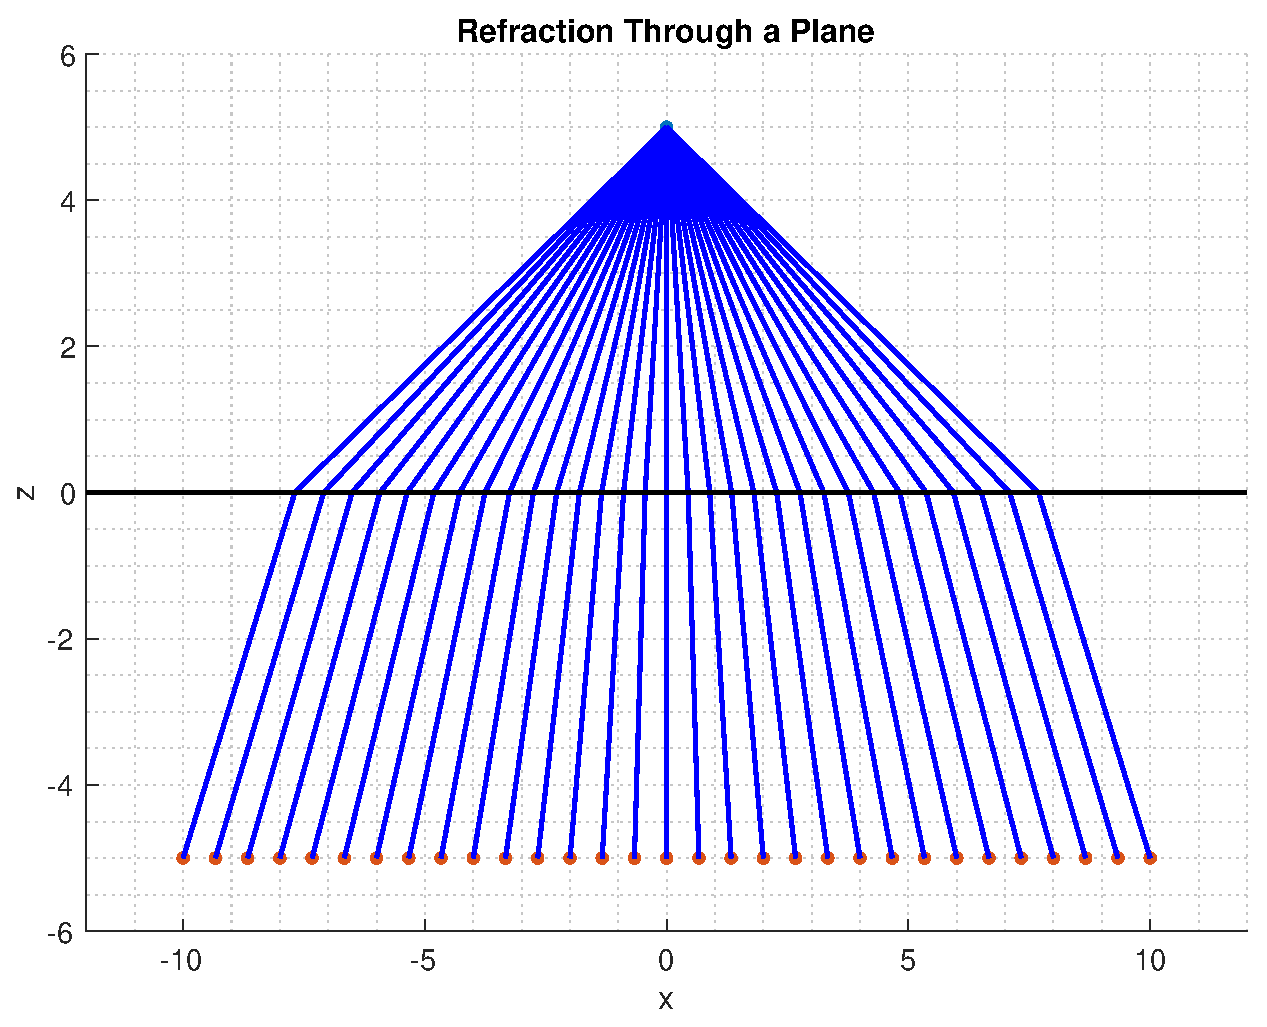
\includegraphics[width=3.5in]{ReflectionRefraction/Figures/refractionraysplane} 
   \caption{Refraction through a plane, $n_1 = 1$, $n_2 = 2$.}
\end{figure}
\subsubsection{Routine}

The routine \texttt{refractionPlane} takes as input the coordinates of $\bb{r}_1$, $\bb{r}_2$, $z_o$, $n_1$ and $n_2$, and returns the coordinates of the refraction point $\bb{r}$ on the interface, the angles $\theta_1$, $\theta_2$, and lengths of the vectors to the refraction point, $l_1$ and $l_2$. The quartic solution is used by default. Use the optional string switch \texttt{'it'} for the iterative solution. For the latter, the routine estimates the required number of iterations by testing a point with the largest free-space $\theta_1$, then applies that number of iterations to all other points in parallel.  The routine is vectorized to take one point, $\bb{r}_1$, while the coordinates of subsurface points, $\bb{r}_2$, can be arrays of any size (all the same size). Outputs are the same size as the $\bb{r}_2$ coordinates. This assumes $n_1$ and $n_2$ are real. The case when $\bb{r}_2$ is at or above the boundary is handled separately. 





{\footnotesize
\VerbatimInput{\code/ReflectionRefraction/refractionPlane.m}
}



\section{Refraction Point - Circular Interface}
We provide two solutions for the refraction point on circular interface. The first is a semi-analytical solution in terms of the roots of a sixth degree polynomial. The second is a vectorized iterative solution that is valid for weak refraction. 



\addtocontents{toc}{\protect\setcounter{tocdepth}{1}}
\subsection{Refraction Point - Circular Interface - Analytical}
\addtocontents{toc}{\protect\setcounter{tocdepth}{2}}

\label{sec:refractdir}
A semi-analytic solution for the refraction point on a circular interface is derived for an arbitrary interior and exterior point. This is based on satisfying Snell's law at the interface. Similar to the quartic solution for the refraction point on a flat surface, the solution is found in terms of the roots of a sixth degree polynomial. An alternative approach is to apply the principle of least action to the total electrical path length of the rays. Both approaches give the same result.

The geometry is shown in Figure \ref{refractthroughcircle}. Let a circle be centered at the origin with radius $r$. The indices of refraction outside and inside the circle are $n_1$ and $n_2$, respectively. Let the exterior and interior points be, $\bb{r}_1$, $\bb{r}_2$, and the refraction point on the circle, $\bb{r}$.  Arbitrary  exterior/interior points are rotated so that the exterior point is aligned with the $y$ axis. Once the refraction point is found in this geometry, it is rotated back. Start with 
\ea{\bb{r}_1 &=& y_1 \hat{y} \\
\bb{r}_2 &=& x_2 \hat{x} + y_2 \hat{y} \\
\bb{r} &=& r_x \hat{x} + r_y \hat{y} }

\noindent where $y_1 > r$ and $r^2 = r_x^2 + r_y^2$.  Also, define the vectors $\bb{v}_1 = \bb{r}_1 - \bb{r}$ and $\bb{v}_2 = \bb{r}_2 - \bb{r}$.  The sine of the incident and transmission angles at the refraction point can be written as the following cross products:
\ea{\sin\theta_1 \hat{z} &=& \dfrac{\bb{r} \times \bb{v}_1}{\vert \bb{r} \vert \vert \bb{v}_1\vert } \\
\sin\theta_2 \hat{z} &=& \dfrac{(-\bb{r}) \times \bb{v}_2}{\vert \bb{r} \vert \vert \bb{v}_2\vert }  }

\begin{figure}[h] 
   \centering
   \includegraphics[width=2.5in]{ReflectionRefraction/Figures/refractionCircle} 
   \caption{Geometry for refraction through a circle. }
   \label{refractthroughcircle}
\end{figure}

Equating through Snell's law, expanding the cross products, and squaring both sides, we get 
\eq{\dfrac{r_x^2 y_1^2}{r_x^2 + (y_1-r_y)^2} = \left(\dfrac{n_2}{n_1}\right)^2 \dfrac{(r_xy_2 - r_y x_2)^2}{(x_2 - r_x)^2 + (y_2-r_y)^2}} 

Next, expand the squares, substitute $r_y^2 = r^2 - r_x^2$, and collect terms to get 

%\eq{\dfrac{r_x^2 y_1^2}{r_x^2 + r_y^2 - 2r_y y_1 + y_1^2} = \left(\dfrac{n_2}{n_1}\right)^2 \dfrac{(r_xy_2 - r_y x_2)^2}{x_2^2 - 2x_2r_x + r_x^2 + r_y^2 - 2r_y y_2 + y_2^2}} 
%
%\eq{\dfrac{(n_1^2/n_2^2)  y_1^2r_x^2 }{r^2 - 2r_y y_1 + y_1^2} =   \dfrac{ r_x^2y_2^2 -2r_y x_2r_xy_2 +  (r^2 - r_x^2) x_2^2}{x_2^2 - 2x_2r_x + r^2 - 2r_y y_2 + y_2^2}} 
%
%\eq{\dfrac{(n_1^2/n_2^2)  y_1^2r_x^2}{r^2+ y_1^2 - 2 y_1r_y } =   \dfrac{ (y_2^2 -  x_2^2)r_x^2 -2 x_2y_2r_yr_x +  r^2x_2^2  }{x_2^2 + y_2^2+ r^2 - 2x_2 r_x  - 2y_2 r_y }} 

\eq{\dfrac{c_1 r_x^2}{c_2  + c_3 r_y } =   \dfrac{ c_4 r_x^2 + c_5 r_yr_x +  c_6 }{c_7 + c_8 r_x  + c_9 r_y }} 

\noindent where $c_n = \left\{(n_1^2/n_2^2)  y_1^2, r^2+ y_1^2, - 2y_1, y_2^2 -  x_2^2, -2 x_2y_2, r^2x_2^2, x_2^2 + y_2^2+ r^2, - 2x_2, - 2y_2\right\}, n = 1... 9$. To proceed, multiply through by the denominators, substitute $r_y^2$ again where it occurs, and collect $r_y$ on one side of the equation, then 
\eq{b_1 r_x^3 + b_2 r_x^2  + b_3 r_x +b_4 = (b_5 r_x^2 + b_6 r_x + b_7 )r_y}

\noindent where $b_n = \left\{c_3 c_5 + c_1 c_8,  c_1 c_7 - c_2 c_4, -c_3 c_5 r^2, -c_2c_6, c_3c_4 - c_1 c_9, c_2c_5, c_3c_6\right\}, n = 1...7$.  Squaring both sides once more, substituting $r_y^2$ a third time, this can be written as a sixth degree polynomial in $r_x$ as
\eq{\sum_{n=0}^6 a_n r_x^n = 0}
\ea{a_6 &=& b_1^2 + b_5^2  \\
a_5 &=& 2 b_1 b_2 + 2 b_5 b_6  \\
a_4 &=&  b_2^2 - b_5^2 r^2 + 2 b_7 b_5 + b_6^2 + 2 b_1 b_3  \\
a_3 &=& - 2 b_5 b_6 r^2 + 2 b_1 b_4 + 2 b_2 b_3 + 2 b_6 b_7 \\
a_2 &=& b_3^2 - b_6^2 r^2 + b_7^2 - 2 b_5 b_7 r^2 + 2 b_2 b_4 \\ 
a_1 &=& - 2 b_6 b_7 r^2 + 2 b_3 b_4 \\
a_0 &=& b_4^2 - b_7^2 r^2 }

%\ea{c_1 &=& (n_1^2/n_2^2)  y_1^2  \\
%c_2 &=&  r^2+ y_1^2  \\
%c_3 &=& - 2y_1 \\
%c_4&=& y_2^2 -  x_2^2 \\ 
%c_5&=& -2 x_2y_2 \\
%c_6 &=& r^2x_2^2  \\
%c_7 &=& x_2^2 + y_2^2+ r^2 \\
%c_8 &=& - 2x_2 \\
%c_9 &=& - 2y_2}
%\ea{b_1 &=& c_3 c_5 + c_1 c_8  \\
%b_2 &=&  c_1 c_7 - c_2 c_4  \\
%b_3 &=& -c_3 c_5 r^2 \\
%b_4&=& -c_2c_6 \\ 
%b_5 &=& c_3c_4 - c_1 c_9 \\
%b_6 &=& c_2c_5  \\
%b_7 &=& c_3c_6 }

%\ea{a_6 &=& b_1^2 + b_5^2  \\
%a_5 &=& 2 b_1 b_2 + 2 b_5 b_6  \\
%a_4 &=&  b_2^2 - b_5^2 r^2 + 2 b_7 b_5 + b_6^2 + 2 b_1 b_3  \\
%a_3 &=& - 2 b_5 b_6 r^2 + 2 b_1 b_4 + 2 b_2 b_3 + 2 b_6 b_7 \\
%a_2 &=& b_3^2 - b_6^2 r^2 + b_7^2 - 2 b_5 b_7 r^2 + 2 b_2 b_4 \\ 
%a_1 &=& - 2 b_6 b_7 r^2 + 2 b_3 b_4 \\
%a_0 &=& b_4^2 - b_7^2 r^2 }

Once the roots are computed, they are sifted to find the valid solution, because squaring twice created extraneous solutions. Roots with a non-zero imaginary part are rejected. Then $r_y$ is computed and only solutions that satisfy Snell's law at the boundary are kept. In the event of a tie, the refraction point that gives the smallest electrical distance is kept, consistent with the principle of least action. Finally, we check that $\theta_1 < \pi/2$ to make sure the ray does not pass through the circle twice (this angle is computed with the dot product of $\bb{r}$ and $\bb{v}_1$ to safely handle $\pm \hat{x}$ solutions). 


\begin{figure}[h] 
   \centering
   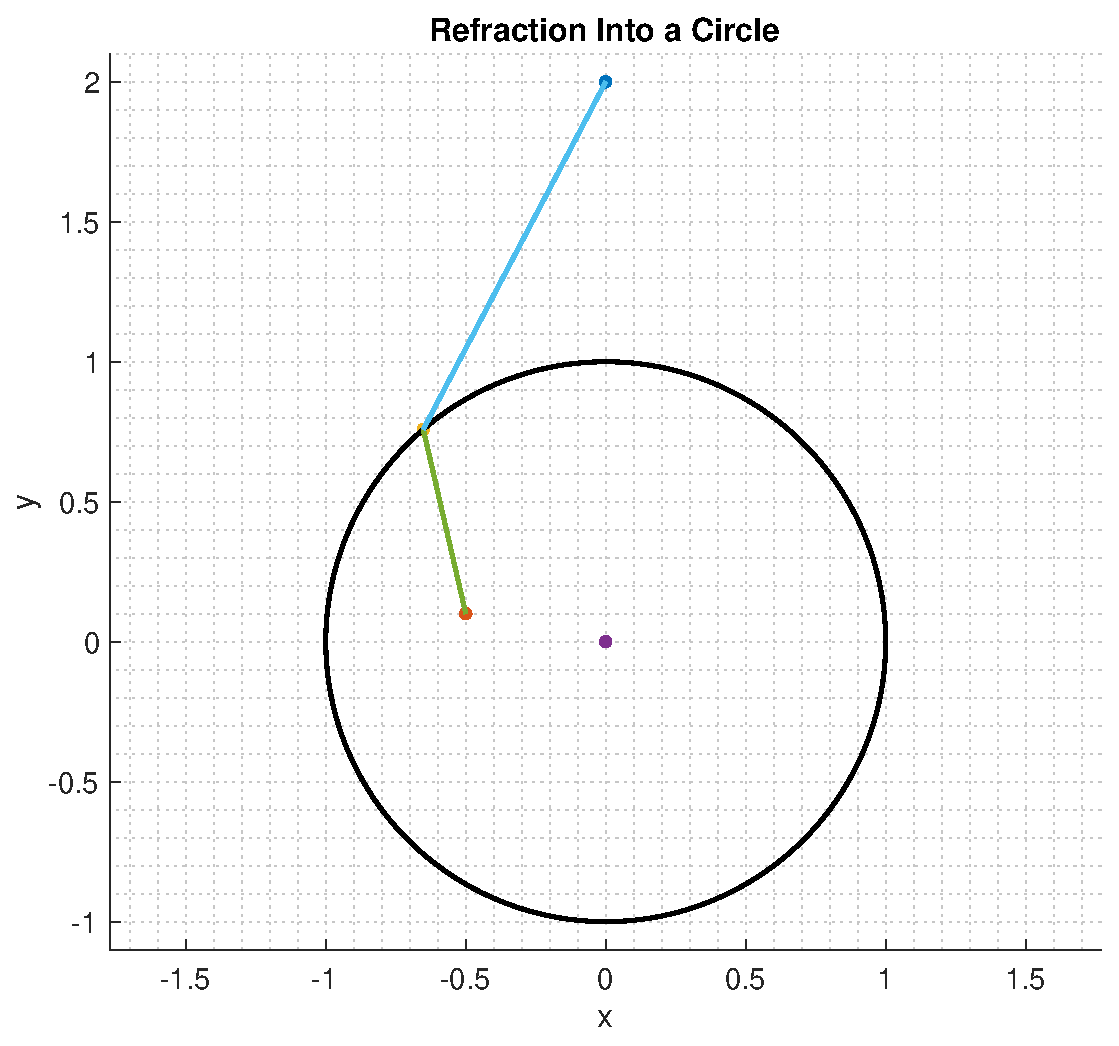
\includegraphics[width=3.5in]{ReflectionRefraction/Figures/refractionrayscircle} 
   \caption{Refraction into a circle between two points. Exterior index of refraction $n_1 = 1$, interior index of refraction $n_2 = 2$, and radius $r = 1$. }
\end{figure}


The routine \texttt{refractionCircle} takes as input the coordinates of an arbitrary exterior point, $\bb{r}_1$, an arbitrary interior point, $\bb{r}_2$, index of refractions $n_1$, $n_2$ and radius $r$, and returns the coordinates of the refraction point on the circle, the incident and transmission angles $\theta_1$ and $\theta_2$ in radians, and the magnitudes of the vectors $\bb{v}_1$ and $\bb{v}_2$. It first rotates the points to align them with the $y$ axis. It returns \texttt{nan} if no solution exists. It also assumes $n_1$ and $n_2$ are real.  Because this relies on \texttt{roots} it is not vectorized. 

{\footnotesize
\VerbatimInput{\code/ReflectionRefraction/refractionCircle.m}
}

%
%\newpage
%
%\section{Refraction Point - Circular Interface}
%
%\ea{\bb{r}_1 &=& x_1 \hat{x} + y_1 \hat{y} \\
%\bb{r}_2 &=& x_2 \hat{x} + y_2 \hat{y} \\
%\bb{r} &=& r_x \hat{x} + r_y \hat{y} }
%
%\noindent where $r^2 = r_x^2 + r_y^2$.  Define the vectors
%\ea{\bb{v}_1 &=& \bb{r}_1 - \bb{r} \\
%\bb{v}_2 &=& \bb{r}_2 - \bb{r} }
%
%The total electrical path length is 
%\eq{L = n_1 v_1 + n_2 v_2}
%
%We want the point $(r_x,r_y)$ that gives the minimum of $L$.  Writing out the magnitudes of the vectors, substituting $r_y = \sqrt{r^2 + r_x^2}$, differentiating with respect to $r_x$, setting the derivative to zero, moving one term to the other side of the equation, squaring both sides, and collecting terms, one can arrive at 
%
%\eq{\dfrac{ c_1 r_x^2 + c_2 r_x \sqrt{r^2 - r_x^2}  + c_3}{c_4 r_x + c_5 \sqrt{r^2 - r_x^2} + c_6} = \dfrac{c_7 r_x^2 + c_8 r_x   \sqrt{r^2 - r_x^2}+ c_9}{c_{10} r_x + c_{11} \sqrt{r^2 - r_x^2} + c_{12}}}
%
%\ea{c_1 &=& n_1^2 x_1^2 - n_1^2 y_1^2 \\
%c_2 &=& 2 n_1^2 x_1 y_1 \\
%c_3 &=& -n_1^2 r^2 x_1^2 \\
%c_4 &=& 2 x_1 \\
%c_5 &=& 2 y_1 \\
%c_6 &=& -r^2 - x_1^2 - y_1^2 \\
%}
%
%\noindent where $c_7...c_{12}$ are the same as $c_1...c_6$ except subscript 1 is changed to 2.  Next, multiplying through by the denominators, simplifying, and collecting factors of $r_x$ and $\sqrt{r^2 - r_x^2}$, one can get 
%\eq{b_1 r_x^3 + b_2 r_x^2 + b_3 r_x + b_4 = 
%(b_5 r_x^2  + b_6 r_x + b_7) \sqrt{r^2 - r_x^2}}
%
%\ea{b_1 &=& c_1 c_{10} - c_4 c_7 - c_2 c_{11} + c_5 c_8 \\
%b_2 &=& c_1 c_{12} - c_6 c_7\\
%b_3 &=& c_3 c_{10} - c_4 c_9 + (c_2 c_{11} - c_5 c_8) r^2\\
%b_4 &=& c_3 c_{12} - c_6 c_9\\
%b_5 &=& c_4 c_8 + c_5 c_7 - c_1 c_{11} - c_2 c_{10}\\
%b_6 &=& c_6 c_8 - c_2 c_{12}\\
%b_7 &=& c_5 c_9 - c_3 c_{11}}
%
%Finally, squaring both sides again and collecting powers of $r_x$, this can be written as a sixth degree polynomial as
%
%\eq{\sum_{n=0}^6 a_n r_x^n = 0}
%\ea{a_6 &=& b_1^2 + b_5^2  \\
%a_5 &=& 2 (b_1 b_2 + b_5 b_6)\\
%a_4 &=& b_2^2 - b_5^2 r^2 + 2 b_7 b_5 + b_6^2 + 2 b_1 b_3\\
%a_3 &=& 2 (-b_5 b_6 r^2 + b_1 b_4 + b_2 b_3 + b_6 b_7)\\
%a_2 &=& 2 b_2 b_4 - r^2 (b_6^2 + 2 b_5 b_7) + b_3^2 + b_7^2\\
%a_1 &=& 2 (-b_6 b_7 r^2 + b_3 b_4)\\
%a_0 &=& b_4^2 - b_7^2 r^2 }
%
%(This was all done with a symbolic tool of course). Once the roots are found, they need to be sifted to find the valid solution, because the effect of squaring twice has introduced extraneous solutions. Roots with an imaginary part are rejected. Then $r_y$ is computed and then $\sin(\theta_1)$ and $\sin(\theta_2)$ are computed from the cross products of the vectors. Only solutions that satisfy Snell's law are kept. In the event of a tie, the refraction point that gives the smallest electrical distance is kept, consistent with the principle of least action. Finally, we check that $\theta_1 < \pi/2$ to make sure the ray does not pass through the circle twice, where the angle is computed with the dot product of $\bb{r}$ and $\bb{v}_1$ to safely handle $\pm$ coordinate solutions.  


\addtocontents{toc}{\protect\setcounter{tocdepth}{1}}
\subsection{Refraction Point - Circular Interface - Iterative}
\addtocontents{toc}{\protect\setcounter{tocdepth}{2}}

\label{sec:refractit}
While the solution for refraction through a circular interface in the previous section is exact, the code could not be vectorized because it required the roots of a sixth degree polynomial. However, like the planar interface, a vectorized iterative solution can be derived. Its validity is restricted to mild refraction and small angles but it is lightning fast when it works. The primary application for this is subsurface SAR focusing in, for instance, radar sounding through ice at planetary bodies, where the body curvature needs to be included in the refraction for a large number of subsurface focal points.  

Using the geometry in Figure \ref{refractthroughcircle}, define:
\ea{h &=& y_1 - r \\
d &=& r - y_2}

Using the fact that 
\eq{\sin\theta_1 = \dfrac{r + h}{r}\sin\theta_l}

we can build an iteration as
\begin{eqnarray}
\textrm{Initialize:} \quad \quad \theta_l &\leftarrow &\arctan\left( \dfrac{x_2}{h + d}\right) \ \nonumber \\
\textrm{Iterate:} \quad \quad\theta_1 &\leftarrow &\arcsin\left( \dfrac{r + h}{r}\sin\theta_l \right) \nonumber  \\
\theta_2  &\leftarrow & \arcsin\left( \dfrac{n_2}{n_1} \sin\theta_1 \right) \\
\theta_p  &\leftarrow & \theta_2 - (\theta_1 - \theta_l) \\
(r_x, r_y) &\leftarrow & \textrm{ComputeIntersection}(\theta_p) \\
\theta_l  &\leftarrow &  \arctan\left( \dfrac{r_x}{h + r  - r_y}\right) \nonumber
\end{eqnarray}

\noindent where $\theta_p$ is the angle from the perpendicular at the refraction point to the interior point, and $\textrm{ComputeIntersection}(\theta_p)$ computes the point at which a line from the interior point with slope corresponding to $\theta_p$ intersects the circle.  

This iteration starts with the straight ray approximation for the look angle $\theta_l$ from which it computes the incident angle on the circle, $\theta_1$. With this, the transmission angle, $\theta_2$, is computed via Snell's law. Next, $\theta_p$ is the portion of $\theta_2$ relative to the perpendicular.  Using this, we project a line from the interior point to intersect the circle. The slope of the line corresponds to the angle $\theta_p$. With the new point on the circle, the look angle is computed again and the process repeats.  This is again a Newton iteration of the transcendental solution for one of the variables. As before, the solution is not the most robust and should be used when the refraction is mild.

\begin{figure}[h] 
   \centering
   \subfigure{\includegraphics[width=2in]{ReflectionRefraction/Figures/refractioncirclethetap}}
   \subfigure{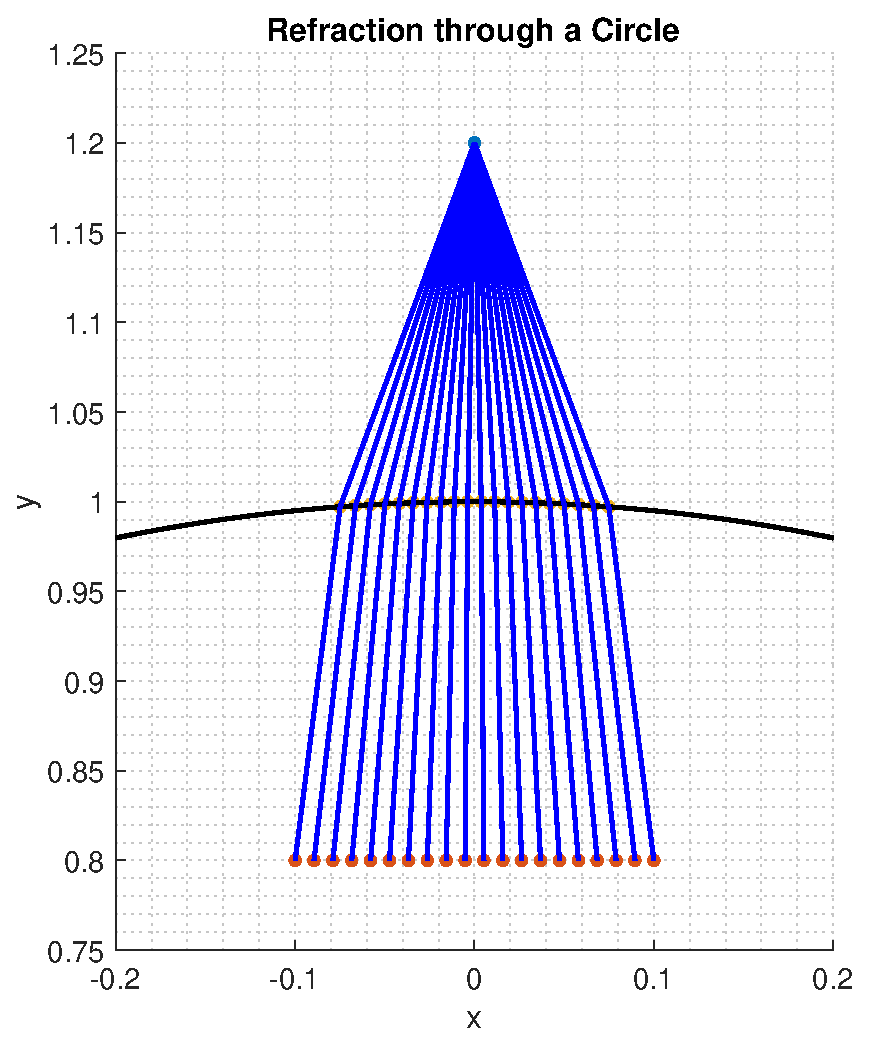
\includegraphics[width=3in]{ReflectionRefraction/Figures/refractionrayscircleiterative}}
   \caption{Left: Angles at the refraction point for iterative solution. Right:Refraction into a circle between multiple points using the vectorized iterative solution. Exterior index of refraction $n_1 = 1$, interior index of refraction $n_2 = 2$, and radius $r = 1$.  }
\end{figure}



%
%\begin{figure}[h] 
%   \centering
%   \includegraphics[width=2in]{ReflectionRefraction/Figures/refractioncirclethetap} 
%   \caption{Angles at the refraction point for iterative solution.}
%\end{figure}
%
%
%\begin{figure}[h] 
%   \centering
%   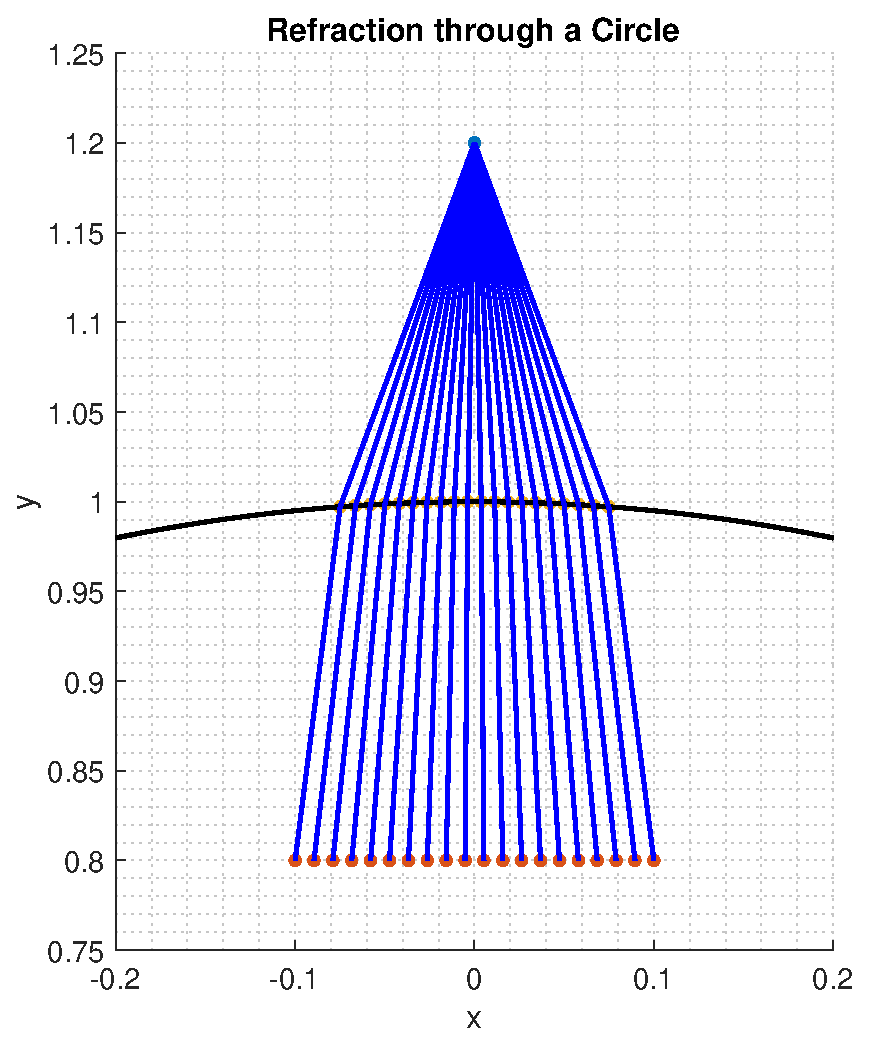
\includegraphics[width=3in]{ReflectionRefraction/Figures/refractionrayscircleiterative} 
%   \caption{Refraction into a circle between multiple points using the vectorized iterative solution. Exterior index of refraction $n_1 = 1$, interior index of refraction $n_2 = 2$, and radius $r = 1$. }
%\end{figure}


\clearpage
\paragraph{Intersection of Circle and Line}

Given a line $y = mx + b$ and a circle $(x-p)^2 + (y-q)^2 = r^2$, the point of intersection $(X,Y)$ is found by substituting the first equation into the second and solving the resulting quadratic for $x$:
\begin{eqnarray}
A &=& m^2 + 1 \nonumber \\
B &=& 2(mb - mq - p) \nonumber \\
C &=& q^2 - r^2 + p^2 - 2bq +b^2 \nonumber \\
X &=& \dfrac{-B \pm \sqrt{B^2 - 4AC}}{2A} \nonumber \\
Y &=& mX + b \nonumber
\end{eqnarray}

\paragraph{ComputeIntersection($\theta_p$)}
Let the center of the circle be the origin $(p,q)=(0,0)$. The line with slope corresponding to angle $\theta_p$ passing though the interior point at $(x_2, y_2)$ is given by 
\eq{y = -\cot\theta_p(x - x_2) + y_2  }

The parameters used in the equations above for the intersection of the line and circle are therefore
\begin{eqnarray}
m &=& -\cot \theta_p \nonumber \\
b &=& x_2\cot\theta_p + y_2 \nonumber \\
A &=& m^2 + 1 \nonumber \\
B &=& 2mb \nonumber \\
C &=& -r^2 + b^2 \nonumber 
\end{eqnarray}

For this problem, the choice of quadratic root is determined by the sign of $x_2$. Furthermore, if the $y$ coordinate of the refraction point is negative at any point in the iteration, then the other root is chosen. Points that are collinear with the origin and the source, where there is no refraction, need to be handled separately. Finally, in this geometry, the look angle is given by 
\eq{\tan\theta_l = \dfrac{r_x}{h + r - r_y} }


The routine \texttt{refractionCircleIterative} is a vectorized implementation of the routine above. It takes an input pairs of $\bb{r}_1$, $\bb{r}_2$, the index of refraction $n_1$, $n_2$, radius $r$, and number of iterations, \texttt{nit}, and returns the refraction points, $\bb{r}$, incident and transmission angles $\theta_1$, $\theta_2$, $\theta_l$, and the lengths of the vectors $\bb{v}_1$ and $\bb{v}_2$. The point arrays can be any size. This assumes $n_1$ and $n_2$ are real. This should only be used in its present form for large radii, and depths that are less than or equal to the heights. Set \texttt{nit} to be 10 or larger, it defaults to 40. The algorithm rotates points to align the exterior points to the $y$ axis, to be consistent with the solution as written, then rotates them back.


{\footnotesize
\VerbatimInput{\code/ReflectionRefraction/refractionCircleIterative.m}
}


\section{Refraction Point - Sphere}

We can adapt the solution for the refraction point over a circle to that for an arbitrary interior and exterior points over a sphere.  Let $\bb{r}_1$ be the exterior point, $\bb{r}_2$ be the interior point, and $\bb{r}$ be the point of refraction on the sphere.  The sphere has radius $r$ centered at the origin.  Define a new coordinate system $[\hat{u}, \hat{v}, \hat{w}]$ in the $\bb{r}_1$-$\bb{r}_2$ plane such that 
\ea{\hat{v} &=& \hat{r}_1  \\
\hat{w} &=& \dfrac{\bb{r}_2 \times \hat{v}}{\vert \bb{r}_2 \times \hat{v} \vert }  \\
\hat{u} &=& \hat{v} \times \hat{w} 
}

The exterior and interior points are represented in this frame as
\ea{\bb{r}_1' &=& \vert \bb{r}_1 \vert \hat{v}  \\
\bb{r}_2' &=& \left( \bb{r}_2 \cdot \hat{u}  \right)\hat{u}  + \left( \bb{r}_2 \cdot \hat{v}  \right)\hat{v}   }

The coordinates of $\bb{r}_1'$ and $\bb{r}_2'$ can now be used as inputs to either of the two circular refraction routines from Section \ref{sec:refractdir} or \ref{sec:refractit}. The magnitude of $\bb{r}_1'$ in the $\hat{v}$ direction corresponds to the $y$-coordinate of the exterior point in both routines, while $\left( \bb{r}_2 \cdot \hat{u}  \right) $ and $\left( \bb{r}_2 \cdot \hat{v}  \right)$ correspond to the $x$ and $y$ coordinates, respectively, of the interior point in both routines. Once solved, the $x$ and $y$ coordinates of the refraction point on the 2D circle, $r_x$ and $r_y$, are mapped back to the original 3D frame as 
\eq{ \bb{r} = r_x \hat{u} + r_y \hat{v}}

The routine \texttt{refractionSphere} computes the refraction through a sphere that is centered at the origin. It takes as input the Cartesian coordinates of pairs of exterior and interior points of any array size, the index of refraction for the exterior and interior, $n_1$, $n_2$, respectively, and the radius of the sphere $r$. The outputs are the coordinates of the refraction point on the sphere, incident angle, transmission angle, and look angle which measured from the radial line of the exterior point, as well as the two path lengths inside and outside the sphere. The routine transforms the input coordinates using the mapping above in order to use the circle refraction algorithms, \texttt{refractionCircle} or \texttt{refractionCircleIterative}. The routine defaults to the direct circle refraction solution which loops over each pair of points. The direction solution can also be chosen using the string switch \texttt{'dir'}. Use string switch \texttt{'it'} to select the vectorized iterative circle refraction solution which can also take an optional input argument for the number of iterations.  

\begin{figure}[H] 
   \centering
   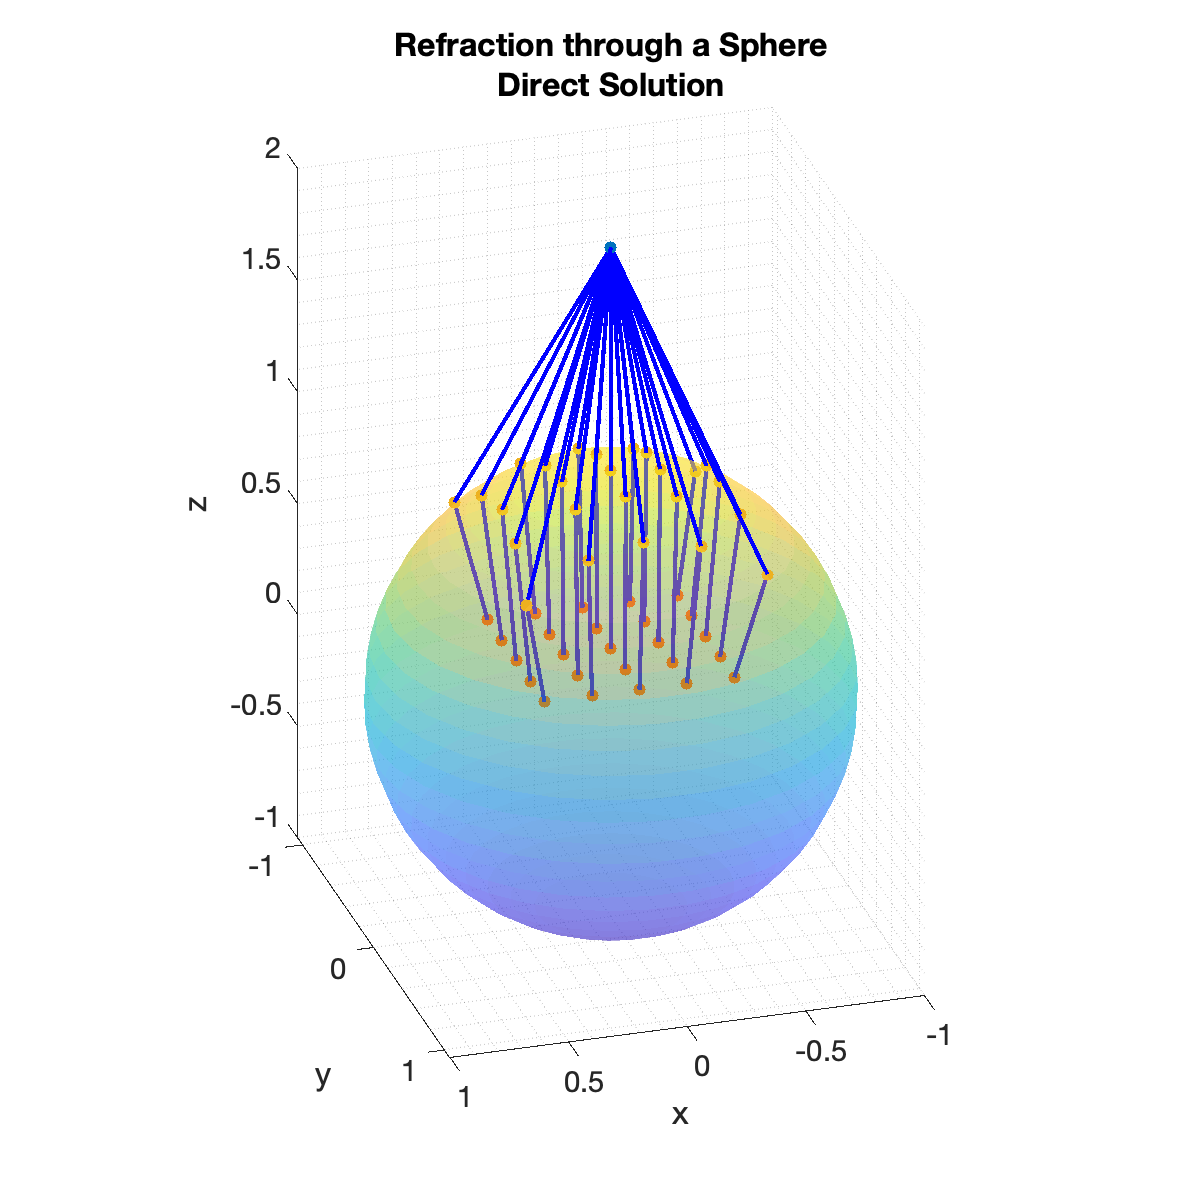
\includegraphics[width=4in]{ReflectionRefraction/Figures/refractionspheredirect} 
   \caption{Refraction into a sphere between multiple points. Exterior index of refraction $n_1 = 1$, interior index of refraction $n_2 = 2$, and sphere radius $r = 1$. }
\end{figure}



{\footnotesize
\VerbatimInput{\code/ReflectionRefraction/refractionSphere.m}
}









